\documentclass[11pt,a4paper]{article}
\usepackage[T1]{fontenc}
\usepackage[utf8]{inputenc}
\usepackage[french]{babel}
\frenchsetup{StandardItemLabels=true}
\usepackage{lmodern}
\usepackage[a4paper,margin=2.4cm]{geometry}
\usepackage{amsmath,amssymb}
\usepackage{booktabs,array}
\usepackage{graphicx}
\usepackage{float}
\usepackage{needspace}
\usepackage[font=small,labelfont=bf]{caption}
\usepackage{xcolor}
\usepackage{fancyhdr}
\usepackage{listings}
\usepackage{tikz}
\usetikzlibrary{positioning}
\usepackage[most]{tcolorbox}
\usepackage[hidelinks]{hyperref}

\definecolor{bleu}{HTML}{1F4E79}
\definecolor{orange}{HTML}{E07B00}
\graphicspath{{figures/}}
\setlength{\parskip}{0.45em}
\setlength{\parindent}{0pt}

\pagestyle{fancy}
\fancyhf{}
\lhead{\small Gestion des stocks d'un supermarché}
\rhead{\small Recherche Opérationnelle, M2 IDEE}
\cfoot{\thepage}

% Encadre "a retenir"
\newtcolorbox{retenir}{colback=bleu!6,colframe=bleu,boxrule=0.6pt,arc=2pt,
  left=6pt,right=6pt,top=4pt,bottom=4pt}

\lstset{language=Python,basicstyle=\ttfamily\footnotesize,
  keywordstyle=\color{bleu}\bfseries,commentstyle=\color{gray},
  stringstyle=\color{orange},frame=single,rulecolor=\color{gray!50},
  breaklines=true,showstringspaces=false}

\AtBeginDocument{\renewcommand{\tablename}{Tableau}}
\newcommand{\eur}{\,\text{€}}

\begin{document}

% ------------------------------------------------------------------ titre
\begin{titlepage}
\centering
{\large Université d'Angers\par}
{\large Master 2 Ingénierie des Données et Évaluations Économétriques\par}
\vspace{3.2cm}
{\large Dossier de Recherche Opérationnelle et Optimisation\par}
{\large Sujet 3 : problème de gestion des stocks\par}
\vspace{0.8cm}
\rule{\linewidth}{1pt}\par
\vspace{0.5cm}
{\huge\bfseries\color{bleu} Gestion des stocks d'un supermarché\par}
\vspace{0.4cm}
{\Large Quand y a-t-il rupture, quand et combien commander,\\[2pt]
comment répartir le stock entre le rayon et la réserve ?\par}
\vspace{0.5cm}
\rule{\linewidth}{1pt}\par
\vspace{1.2cm}
{\large Programmation linéaire et algorithme du simplexe :\\
un cas résolu à la main, puis une application Python\par}
\vspace{3cm}
{\Large Diakhou Mbengue\par}
\vfill
{\large Année universitaire 2026 à 2027\par}
\end{titlepage}

% ------------------------------------------------------------------ resume
\section*{Résumé}
Ce dossier étudie la gestion des stocks d'un supermarché et répond à trois questions :
quand y a-t-il rupture, quand et combien commander, comment répartir le stock entre le rayon
et la réserve. Il utilise les méthodes du cours : programmation linéaire, méthode graphique,
méthode des sommets et algorithme du simplexe.

La démarche se fait en deux temps. Dans la partie 2, les trois questions sont traitées
\textbf{entièrement à la main sur un magasin de deux produits}, ce qui permet de voir chaque
étape : le programme linéaire, la méthode graphique, les trois tableaux du simplexe, puis la
lecture des ruptures, du calendrier de commande et du partage du rayon. Dans la partie 3, la
même démarche est programmée en Python pour obtenir une \textbf{application} qui accepte un
nombre quelconque de produits : elle est vérifiée sur le cas à deux produits, appliquée aux
six produits d'un Super U, puis testée jusqu'à 1\,000 produits.

Sur le cas à six produits, la marge maximale est de 5\,630,55\eur{} par semaine, avec un
budget entièrement dépensé. Les ruptures (lait et yaourts à partir du vendredi soir, eau le
dimanche) coûtent 711,45\eur{} par semaine. Un meilleur partage du rayon rapporte
44,88\eur{} par jour, et un second remplissage quotidien supprime toutes les ventes perdues
en rayon.

\textbf{Application en ligne :} \href{https://projet-ro-stocks.streamlit.app/}{\texttt{https://projet-ro-stocks.streamlit.app/}}\\
Code et rapport : \href{https://github.com/diakhouM/projet-ro-stocks}{\texttt{github.com/diakhouM/projet-ro-stocks}}

\textbf{Mots-clés :} gestion des stocks, programmation linéaire, algorithme du simplexe,
variables d'écart, rupture, rayon, réserve, application Python.

\subsection*{Les chiffres clés}
\begin{center}\small
\begin{tabular}{@{}lrr@{}}
\toprule
 & 2 produits (à la main) & 6 produits (application) \\
\midrule
Marge hebdomadaire maximale & 550\eur & 5\,630,55\eur \\
Nombre de pivots du simplexe « commandes » & 2 & 8 \\
Marge perdue chaque semaine à cause des ruptures & 570\eur & 711,45\eur \\
Marge par jour, rayon actuel $\to$ rayon optimal & 120 $\to$ 130\eur & 806 $\to$ 850,88\eur \\
\bottomrule
\end{tabular}
\end{center}

\newpage
{\setlength{\parskip}{0pt}\small\tableofcontents}
\newpage

% ------------------------------------------------------------------ 1
\section{Introduction}

\subsection{Contexte et problématique}
Dans la grande distribution, le stock est à la fois une nécessité et un coût. S'il est trop
faible, le rayon est vide, la vente est perdue et le client peut changer d'enseigne. S'il est
trop élevé, il immobilise de la trésorerie et occupe une réserve dont la surface est
limitée. Le responsable d'un magasin doit donc répartir des ressources rares, l'argent et la
place, entre des produits qui n'ont ni le même coût, ni le même volume, ni la même marge.

La recherche opérationnelle regroupe les méthodes qui aident à prendre ce type de décision :
modéliser un problème, puis chercher la meilleure solution avec un algorithme. La
programmation linéaire consiste à maximiser une fonction économique linéaire sous des
contraintes linéaires : c'est exactement la forme du problème du magasin. Ce dossier pose
trois questions :
\begin{enumerate}
\item \textbf{Quand y a-t-il rupture ?}
\item \textbf{Quand et combien commander ?}
\item \textbf{Comment répartir le stock entre le rayon et la réserve ?}
\end{enumerate}

\subsection{Démarche : d'abord à la main, ensuite par une application}
Une solution calculée par un programme n'a de valeur que si l'on comprend ce que le
programme fait. Le dossier procède donc en deux temps.

\begin{itemize}
\item \textbf{Partie 2 : un magasin de deux produits, résolu à la main.} Avec deux produits,
  les tableaux du simplexe tiennent sur une page et la méthode graphique se dessine. Les
  trois questions y sont traitées l'une après l'autre.
\item \textbf{Partie 3 : une application Python pour un nombre quelconque de produits.} La
  même démarche est programmée. L'application est d'abord vérifiée sur le cas à deux
  produits, puis appliquée aux six produits d'un Super U (hypothèses imaginaires), puis
  testée sur 10, 100, 300 et 1\,000 produits.
\end{itemize}

\begin{table}[H]
\centering\small
\caption{Les questions du dossier et les méthodes du cours utilisées}\label{tab:demarche}
\begin{tabular}{@{}p{4.3cm}p{7.2cm}l@{}}
\toprule
Question & Méthode & Cours \\
\midrule
Combien commander ? & Programme linéaire « commandes », méthode graphique, méthode des
  sommets, algorithme du simplexe & Chapitre 1 \\
Quand y a-t-il rupture ? & Lecture des variables d'écart du tableau final & Chapitre 1 \\
Quand commander ? & Calendrier construit à partir des délais de livraison & Calcul simple \\
Rayon ou réserve ? & Programme linéaire « rayon », résolu de la même façon & Chapitre 1 \\
\bottomrule
\end{tabular}
\end{table}

% ------------------------------------------------------------------ 2
\newpage
\section{Le cas manuel : un magasin de deux produits}

\subsection{Les données}
Un petit magasin vend deux produits, A et B. Les chiffres sont choisis pour que les calculs
tombent juste. Le magasin est livré le lundi matin et le rayon est rempli une fois par jour,
le matin.

\begin{table}[H]
\centering\small
\caption{Données du magasin à deux produits}\label{tab:donnees2}
\begin{tabular}{@{}lrr@{}}
\toprule
 & Produit A & Produit B \\
\midrule
Demande par jour & 20 & 20 \\
Demande par semaine $H_i = 7\,d_i$ & 140 & 140 \\
Coût d'achat $c_i$ & 2\eur & 4\eur \\
Prix de vente $p_i$ & 5\eur & 9\eur \\
Marge $m_i = p_i - c_i$ & 3\eur & 5\eur \\
Volume $v_i$ & 1 litre & 1 litre \\
Délai de livraison $L_i$ & 2 jours & 3 jours \\
Stock de sécurité $SS_i$ & 20 & 20 \\
Places actuelles en rayon & 15 & 15 \\
\bottomrule
\end{tabular}
\end{table}

Ressources du magasin : \textbf{budget de 400\eur{} par semaine}, \textbf{réserve de
150 litres}, \textbf{rayon de 30 litres} (les 15 + 15 places actuelles).

Servir toute la demande coûterait $2 \times 140 + 4 \times 140 = 840\eur$ et occuperait
280 litres : c'est plus que le budget et la réserve. Le magasin ne peut donc pas tout
commander, et il faut choisir quoi commander en priorité.

\subsection{Combien commander ?}

\subsubsection*{Le programme linéaire}
On note $a$ et $b$ les quantités de A et de B commandées pour la semaine.
\begin{align*}
\max\; Z &= 3a + 5b && \text{(fonction économique : marge de la semaine)}\\
\text{SC :}\quad 2a + 4b &\le 400 && \text{(budget)}\\
a + b &\le 150 && \text{(réserve)}\\
a \le 140,\quad b &\le 140 && \text{(plafonds : on ne vend pas plus que la demande)}\\
a,\; b &\ge 0
\end{align*}

\subsubsection*{Méthode graphique et méthode des sommets}
\begin{figure}[H]
\centering
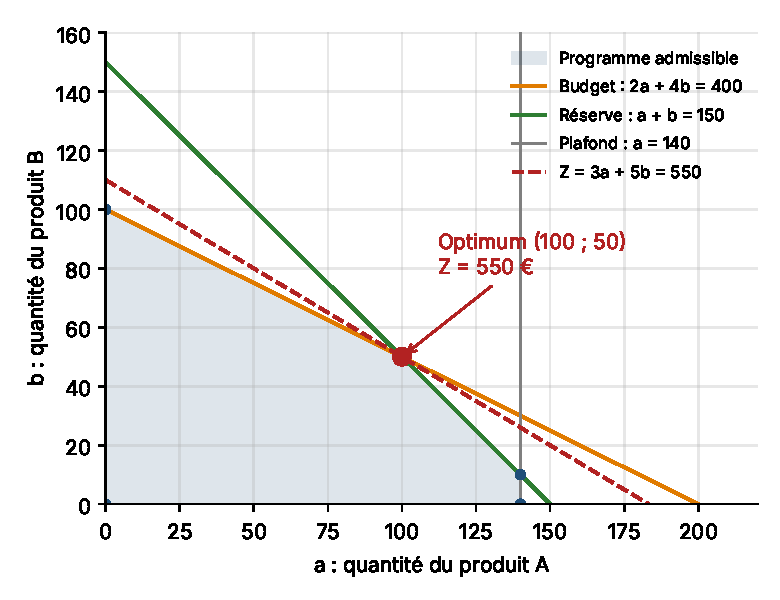
\includegraphics[width=0.62\linewidth]{methode_graphique.pdf}
\caption{Méthode graphique : programme admissible et optimum}\label{fig:graphique}
\end{figure}

Le programme admissible est le polygone grisé de la figure~\ref{fig:graphique}. On déplace
la droite $Z = 3a + 5b$ parallèlement à elle-même, le plus loin possible de l'origine : elle
quitte le programme admissible au point $(100 ; 50)$. La méthode des sommets confirme ce
résultat, car la solution optimale est en l'un des sommets du programme admissible :

\begin{center}\small
\begin{tabular}{@{}lccccc@{}}
\toprule
Sommet & $O(0 ; 0)$ & $A(140 ; 0)$ & $B(140 ; 10)$ & $C(100 ; 50)$ & $D(0 ; 100)$ \\
\midrule
Valeur de $Z$ & 0 & 420 & 470 & \textbf{550} & 500 \\
\bottomrule
\end{tabular}
\end{center}

Le sommet $C$ est à l'intersection du budget et de la réserve : $a + b = 150$ et
$2a + 4b = 400$ donnent $b = 50$ et $a = 100$. Solution optimale :
$(Z^{*} ; a^{*} ; b^{*}) = (550 ; 100 ; 50)$.

\subsubsection*{Algorithme du simplexe}
On intègre les variables d'écart $e_1$ (budget non dépensé), $e_2$ (litres libres en
réserve), $e_3$ et $e_4$ (demande de A et de B non servie). La solution réalisable de base
initiale, où l'on ne commande rien, est
$S_0 = (Z ; a ; b ; e_1 ; e_2 ; e_3 ; e_4) = (0 ; 0 ; 0 ; 400 ; 150 ; 140 ; 140)$. À chaque
étape, la variable entrante est celle dont le profit marginal $\Delta_j$ est le plus grand,
et la variable sortante celle dont le rapport $b_i / a_{ij}$ est le plus petit
(uniquement pour les $a_{ij}$ strictement positifs).

{\footnotesize
\Needspace{9\baselineskip}
\textbf{Tableau 1} : $b$ entre ($\Delta = 5$), $e_1$ sort (rapport 100), le pivot est 4.
\begin{center}
\begin{tabular}{@{}cc|rrrrrr|r|r@{}}
\toprule
$c_B$ & Base & $a$ & $b$ & $e_1$ & $e_2$ & $e_3$ & $e_4$ & $b_i$ & Rapport \\
\midrule
0 & $e_1$ & 2 & \textbf{4} & 1 & 0 & 0 & 0 & 400 & \textbf{100} \\
0 & $e_2$ & 1 & 1 & 0 & 1 & 0 & 0 & 150 & 150 \\
0 & $e_3$ & 1 & 0 & 0 & 0 & 1 & 0 & 140 & \\
0 & $e_4$ & 0 & 1 & 0 & 0 & 0 & 1 & 140 & 140 \\
\midrule
 & $\Delta_j$ & 3 & \textbf{5} & 0 & 0 & 0 & 0 & 0 & \\
\bottomrule
\end{tabular}
\end{center}
\Needspace{9\baselineskip}
\textbf{Tableau 2} : $S_1 = (500 ; 0 ; 100 ; 0 ; 50 ; 140 ; 40)$ ; $a$ entre
($\Delta = 0{,}5$), $e_2$ sort (rapport 100), le pivot est 0,5.
\begin{center}
\begin{tabular}{@{}cc|rrrrrr|r|r@{}}
\toprule
$c_B$ & Base & $a$ & $b$ & $e_1$ & $e_2$ & $e_3$ & $e_4$ & $b_i$ & Rapport \\
\midrule
5 & $b$ & 0,5 & 1 & 0,25 & 0 & 0 & 0 & 100 & 200 \\
0 & $e_2$ & \textbf{0,5} & 0 & $-0{,}25$ & 1 & 0 & 0 & 50 & \textbf{100} \\
0 & $e_3$ & 1 & 0 & 0 & 0 & 1 & 0 & 140 & 140 \\
0 & $e_4$ & $-0{,}5$ & 0 & $-0{,}25$ & 0 & 0 & 1 & 40 & \\
\midrule
 & $\Delta_j$ & \textbf{0,5} & 0 & $-1{,}25$ & 0 & 0 & 0 & $-500$ & \\
\bottomrule
\end{tabular}
\end{center}
\Needspace{9\baselineskip}
\textbf{Tableau 3} : tous les $\Delta_j$ sont négatifs ou nuls, la solution est optimale.
\begin{center}
\begin{tabular}{@{}cc|rrrrrr|r@{}}
\toprule
$c_B$ & Base & $a$ & $b$ & $e_1$ & $e_2$ & $e_3$ & $e_4$ & $b_i$ \\
\midrule
5 & $b$ & 0 & 1 & 0,5 & $-1$ & 0 & 0 & 50 \\
3 & $a$ & 1 & 0 & $-0{,}5$ & 2 & 0 & 0 & 100 \\
0 & $e_3$ & 0 & 0 & 0,5 & $-2$ & 1 & 0 & 40 \\
0 & $e_4$ & 0 & 0 & $-0{,}5$ & 1 & 0 & 1 & 90 \\
\midrule
 & $\Delta_j$ & 0 & 0 & $-1$ & $-1$ & 0 & 0 & $-550$ \\
\bottomrule
\end{tabular}
\end{center}
}

La solution optimale est $S^{*} = (550 ; 100 ; 50 ; 0 ; 0 ; 40 ; 90)$, identique à celle des
deux méthodes précédentes : \textbf{il faut commander 100 unités de A et 50 unités de B},
pour une marge de 550\eur{} par semaine. Le budget et la réserve sont saturés
($e_1 = e_2 = 0$). Comme les profits marginaux des variables hors base ($e_1$ et $e_2$) sont
non nuls, la solution est unique.

\subsection{Quand y a-t-il rupture ?}
Les variables d'écart $e_3 = 40$ et $e_4 = 90$ du tableau final donnent la réponse : ce sont
les quantités de la demande hebdomadaire qui ne seront pas servies. Il y a rupture dès que le
stock commandé est épuisé. Avec une demande de 20 par jour, la commande tient
$x_i^{*} / d_i$ jours :
\[
\text{produit A : } \frac{100}{20} = 5 \text{ jours},
\qquad
\text{produit B : } \frac{50}{20} = 2{,}5 \text{ jours}.
\]
La livraison arrivant le lundi matin, le produit A est servi du lundi au vendredi et manque
\textbf{à partir du samedi}. Le produit B manque \textbf{à partir du mercredi}.

La marge perdue est $40 \times 3 + 90 \times 5 = 120 + 450 = 570\eur$ par semaine. On le
vérifie : servir toute la demande rapporterait $3 \times 140 + 5 \times 140 = 1\,120\eur$, et
$1\,120 - 550 = 570$.

\begin{retenir}
\textbf{À retenir.} Ces ruptures sont le prix des ressources limitées. Le budget favorise A
(1,5\eur{} de marge par euro dépensé, contre 1,25\eur{} pour B), tandis que la réserve favorise
B (5\eur{} de marge par litre, contre 3\eur{} pour A). Le mélange optimal $(100 ; 50)$ est celui
qui épuise les deux ressources à la fois ; aucun des deux produits ne peut être servi
entièrement.
\end{retenir}

\subsection{Quand commander ?}
Le programme donne les quantités ; la date dépend du délai de livraison. Pour que la
marchandise soit en réserve le lundi matin, il faut commander $L_i$ jours avant : le
produit A (2 jours) se commande \textbf{le samedi} précédent, le produit B (3 jours)
\textbf{le vendredi}.

Entre deux livraisons, un seuil d'alerte permet de réagir : si le stock descend sous le
point de commande $s_i = d_i\,L_i + SS_i$ (la demande pendant le délai, plus le stock de
sécurité), une commande doit déjà être en route. Ici $s_A = 20 \times 2 + 20 = 60$ et
$s_B = 20 \times 3 + 20 = 80$.

\subsection{Rayon ou réserve ?}

\subsubsection*{Le problème}
La marchandise livrée va en réserve, mais le client ne se sert que dans le rayon, rempli une
fois par jour. Avec 15 places pour chaque produit, on ne vend que 15 unités de A et 15
unités de B par jour, alors que la demande est de 20 : la marge est de
$3 \times 15 + 5 \times 15 = 120\eur$ par jour, même si la réserve est pleine. Comment
partager les 30 litres du rayon ?

\subsubsection*{Le programme linéaire}
On note $r_A$ et $r_B$ le nombre de places de chaque produit, et $n$ le nombre de
remplissages par jour (d'abord $n = 1$) : on vend au plus $n\,r_i$ unités par jour.
\begin{align*}
\max\; Z &= 3\,n\,r_A + 5\,n\,r_B && \text{(marge vendue par jour)}\\
\text{SC :}\quad r_A + r_B &\le 30 && \text{(volume du rayon)}\\
n\,r_A \le 20,\quad n\,r_B &\le 20 && \text{(inutile d'exposer plus que la demande)}\\
r_A,\; r_B &\ge 0
\end{align*}

\begin{figure}[H]
\centering
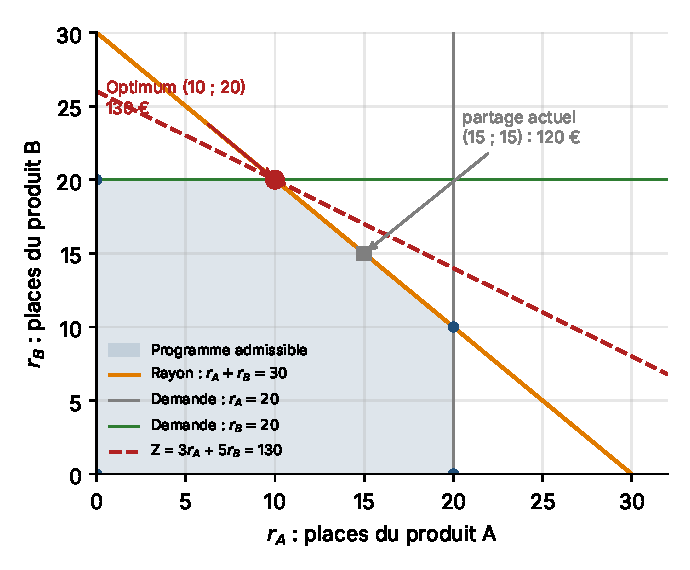
\includegraphics[width=0.52\linewidth]{rayon_2_produits.pdf}
\caption{Partage du rayon pour $n = 1$ : programme admissible, partage actuel et optimum}
\label{fig:rayon2}
\end{figure}

Les sommets du programme admissible sont $(0 ; 0)$, $(20 ; 0)$, $(20 ; 10)$, $(10 ; 20)$ et
$(0 ; 20)$, avec $Z = 0$, $60$, $110$, $\mathbf{130}$ et $100$. L'optimum est $(10 ; 20)$.

\subsubsection*{Le simplexe en deux pivots}
Variables d'écart : $e_1$ (litres libres dans le rayon), $e_2$ et $e_3$ (demande de A et de B
non couverte).

{\footnotesize
\Needspace{9\baselineskip}
\textbf{Tableau 1} : $r_B$ entre ($\Delta = 5$), $e_3$ sort (rapport 20), le pivot est 1.
\begin{center}
\begin{tabular}{@{}cc|rrrrr|r|r@{}}
\toprule
$c_B$ & Base & $r_A$ & $r_B$ & $e_1$ & $e_2$ & $e_3$ & $b_i$ & Rapport \\
\midrule
0 & $e_1$ & 1 & 1 & 1 & 0 & 0 & 30 & 30 \\
0 & $e_2$ & 1 & 0 & 0 & 1 & 0 & 20 & \\
0 & $e_3$ & 0 & \textbf{1} & 0 & 0 & 1 & 20 & \textbf{20} \\
\midrule
 & $\Delta_j$ & 3 & \textbf{5} & 0 & 0 & 0 & 0 & \\
\bottomrule
\end{tabular}
\end{center}
\Needspace{9\baselineskip}
\textbf{Tableau 2} : $r_A$ entre ($\Delta = 3$), $e_1$ sort (rapport 10), le pivot est 1.
\begin{center}
\begin{tabular}{@{}cc|rrrrr|r|r@{}}
\toprule
$c_B$ & Base & $r_A$ & $r_B$ & $e_1$ & $e_2$ & $e_3$ & $b_i$ & Rapport \\
\midrule
0 & $e_1$ & \textbf{1} & 0 & 1 & 0 & $-1$ & 10 & \textbf{10} \\
0 & $e_2$ & 1 & 0 & 0 & 1 & 0 & 20 & 20 \\
5 & $r_B$ & 0 & 1 & 0 & 0 & 1 & 20 & \\
\midrule
 & $\Delta_j$ & \textbf{3} & 0 & 0 & 0 & $-5$ & $-100$ & \\
\bottomrule
\end{tabular}
\end{center}
\Needspace{9\baselineskip}
\textbf{Tableau 3} : tous les $\Delta_j$ sont négatifs ou nuls, la solution est optimale.
\begin{center}
\begin{tabular}{@{}cc|rrrrr|r@{}}
\toprule
$c_B$ & Base & $r_A$ & $r_B$ & $e_1$ & $e_2$ & $e_3$ & $b_i$ \\
\midrule
3 & $r_A$ & 1 & 0 & 1 & 0 & $-1$ & 10 \\
0 & $e_2$ & 0 & 0 & $-1$ & 1 & 1 & 10 \\
5 & $r_B$ & 0 & 1 & 0 & 0 & 1 & 20 \\
\midrule
 & $\Delta_j$ & 0 & 0 & $-3$ & 0 & $-2$ & $-130$ \\
\bottomrule
\end{tabular}
\end{center}
}

\textbf{Réponse pour $n = 1$ :} il faut donner \textbf{10 places à A et 20 places à B}. La
marge passe de 120\eur{} à 130\eur{} par jour : le produit B, plus rentable par litre, passe
en priorité. Le rayon est entièrement utilisé ($e_1 = 0$), et il reste $e_2 = 10$ unités de
la demande de A que le rayon ne peut pas servir.

\subsubsection*{Avec deux remplissages par jour}
Si le rayon est rempli deux fois (le matin et à la mi-journée), on vend $2\,r_i$ unités par
jour, et les contraintes de demande deviennent $2\,r_A \le 20$ et $2\,r_B \le 20$. Le
simplexe, avec les mêmes deux pivots, donne $r_A = r_B = 10$ et $Z = 160\eur$ par jour :
toute la demande est servie ($3 \times 20 + 5 \times 20 = 160$). Le rayon n'est plus saturé :
il reste $e_1 = 10$ litres libres, donc l'agrandir serait inutile.

\subsection{Synthèse du cas à deux produits}
\begin{table}[H]
\centering\small
\caption{Les trois réponses pour le magasin à deux produits}\label{tab:synthese2}
\begin{tabular}{@{}p{4.1cm}p{9.2cm}@{}}
\toprule
Question & Réponse \\
\midrule
Quand y a-t-il rupture ? & Le produit A à partir du samedi, le produit B à partir du
  mercredi (570\eur{} de marge perdue par semaine). \\
Combien commander ? & 100 unités de A et 50 unités de B, pour une marge de 550\eur{} par
  semaine. \\
Quand commander ? & A le samedi, B le vendredi, pour une livraison le lundi matin. \\
Rayon ou réserve ? & 10 places pour A et 20 places pour B : la marge passe de 120 à 130\eur{}
  par jour. Avec deux remplissages, 160\eur{} par jour. \\
\bottomrule
\end{tabular}
\end{table}

% ------------------------------------------------------------------ 3
\newpage
\section{L'application Python : un nombre quelconque de produits}

\subsection{Pourquoi une application}
La méthode de la partie 2 s'applique telle quelle à n'importe quel magasin, mais le calcul à
la main devient impossible. Pour $n$ produits, le tableau du simplexe « commandes » compte
$n + 2$ lignes et $2n + 3$ colonnes : 4 lignes et 7 colonnes pour deux produits, 8 lignes et
15 colonnes pour six, 102 lignes et 203 colonnes pour cent, 1\,002 lignes et 2\,003 colonnes
pour mille. Les étapes sont les mêmes ; seule la taille change, et c'est précisément ce
qu'un programme sait faire.

\subsection{Comment elle fonctionne}
L'application reprend, étape par étape, la démarche de la partie 2.

\begin{enumerate}
\item \textbf{Lecture des produits.} Les données sont dans un fichier CSV (une ligne par
  produit) ou dans \texttt{donnees.py}. Colonnes : produit, demande par jour, coût d'achat,
  prix de vente, délai, stock de sécurité, places en rayon, volume.
\item \textbf{Programme « commandes ».} L'application écrit le programme linéaire, le met
  sous forme canonique et le résout par l'algorithme du simplexe.
\item \textbf{Ruptures.} Elle lit les variables d'écart des plafonds et calcule les jours
  couverts $x_i^{*} / d_i$.
\item \textbf{Calendrier.} Elle déduit le jour de commande de chaque délai.
\item \textbf{Programme « rayon ».} Elle écrit et résout le second programme linéaire.
\end{enumerate}

\textbf{Le modèle pour $n$ produits.} Les deux programmes sont ceux de la partie 2, avec
deux ajouts. D'abord un service minimum $s$ : on commande au moins $s \times H_i$ de chaque
produit (70\,\% dans le cas à six produits, 0 dans l'exemple à la main). Ensuite $n$ produits
au lieu de deux.
\begin{align*}
\text{Commandes :}\quad & \max \sum_i m_i\,x_i
  \quad\text{SC :}\quad \sum_i c_i\,x_i \le B,\;\; \sum_i v_i\,x_i \le V,\;\;
  s\,H_i \le x_i \le H_i\\
\text{Rayon :}\quad & \max \sum_i m_i\,n\,r_i
  \quad\text{SC :}\quad \sum_i v_i\,r_i \le S,\;\; n\,r_i \le d_i
\end{align*}
où $B$ est le budget, $V$ la réserve, $S$ le volume du rayon et $n$ le nombre de
remplissages par jour. Pour que le simplexe s'applique directement, on pose
$x_i = s\,H_i + z_i$ avec $z_i \ge 0$ : la quantité $z_i$ est ce que l'on commande
\textit{au-delà} du minimum, et toutes les contraintes deviennent des « $\le$ » à second
membre positif (programme linéaire canonique du cours).

\textbf{Les fichiers.}
\begin{center}\small
\begin{tabular}{@{}p{5.2cm}p{9cm}@{}}
\toprule
Fichier & Rôle \\
\midrule
\texttt{simplexe.py} & l'algorithme du simplexe en tableaux (le même qu'à la main) \\
\texttt{modele.py} & les deux programmes linéaires, les ruptures, le calendrier \\
\texttt{application.py} & lit les produits, répond aux trois questions, affiche \\
\texttt{app\_streamlit.py} & la même application dans le navigateur (interface Streamlit) \\
\texttt{donnees.py} & les produits et les paramètres du cas d'étude \\
\texttt{exemple\_*\_produits.csv} & des fichiers de produits (2 et 6 produits) \\
\bottomrule
\end{tabular}
\end{center}

\textbf{Utilisation.} Quatre commandes suffisent :
\begin{lstlisting}[language=bash]
python application.py --deux-produits          # l'exemple resolu a la main
python application.py                          # les 6 produits du Super U
python application.py --fichier mes_produits.csv
python application.py --aleatoire 100          # 100 produits generes au hasard
\end{lstlisting}
Le budget, la réserve, le service minimum, le volume du rayon et le nombre de remplissages
se changent par des options (\texttt{--budget 9000}, \texttt{--remplissages 2}, etc.). Pour
un petit magasin, l'application affiche tous les tableaux du simplexe ; pour un grand, elle
n'affiche que les résultats principaux.

\textbf{Interface web.} Le fichier \texttt{app\_streamlit.py} propose la même application
dans le navigateur. Elle est en ligne à l'adresse
\href{https://projet-ro-stocks.streamlit.app/}{\texttt{https://projet-ro-stocks.streamlit.app/}} ; pour la lancer sur son propre ordinateur, il
suffit de taper \texttt{python -m streamlit run app\_streamlit.py}. On y choisit le cas
(2 produits, 6 produits, un fichier CSV ou des produits aléatoires), on modifie directement
le tableau des produits, on règle le budget, la réserve, le service minimum et le nombre de
remplissages du rayon avec le menu de gauche, et le calcul se refait aussitôt. Les réponses
aux trois questions sont dans des onglets, et un onglet « Simplexe pas à pas » affiche les
tableaux pour les petits magasins (figure~\ref{fig:streamlit}).

\begin{figure}[H]
\centering
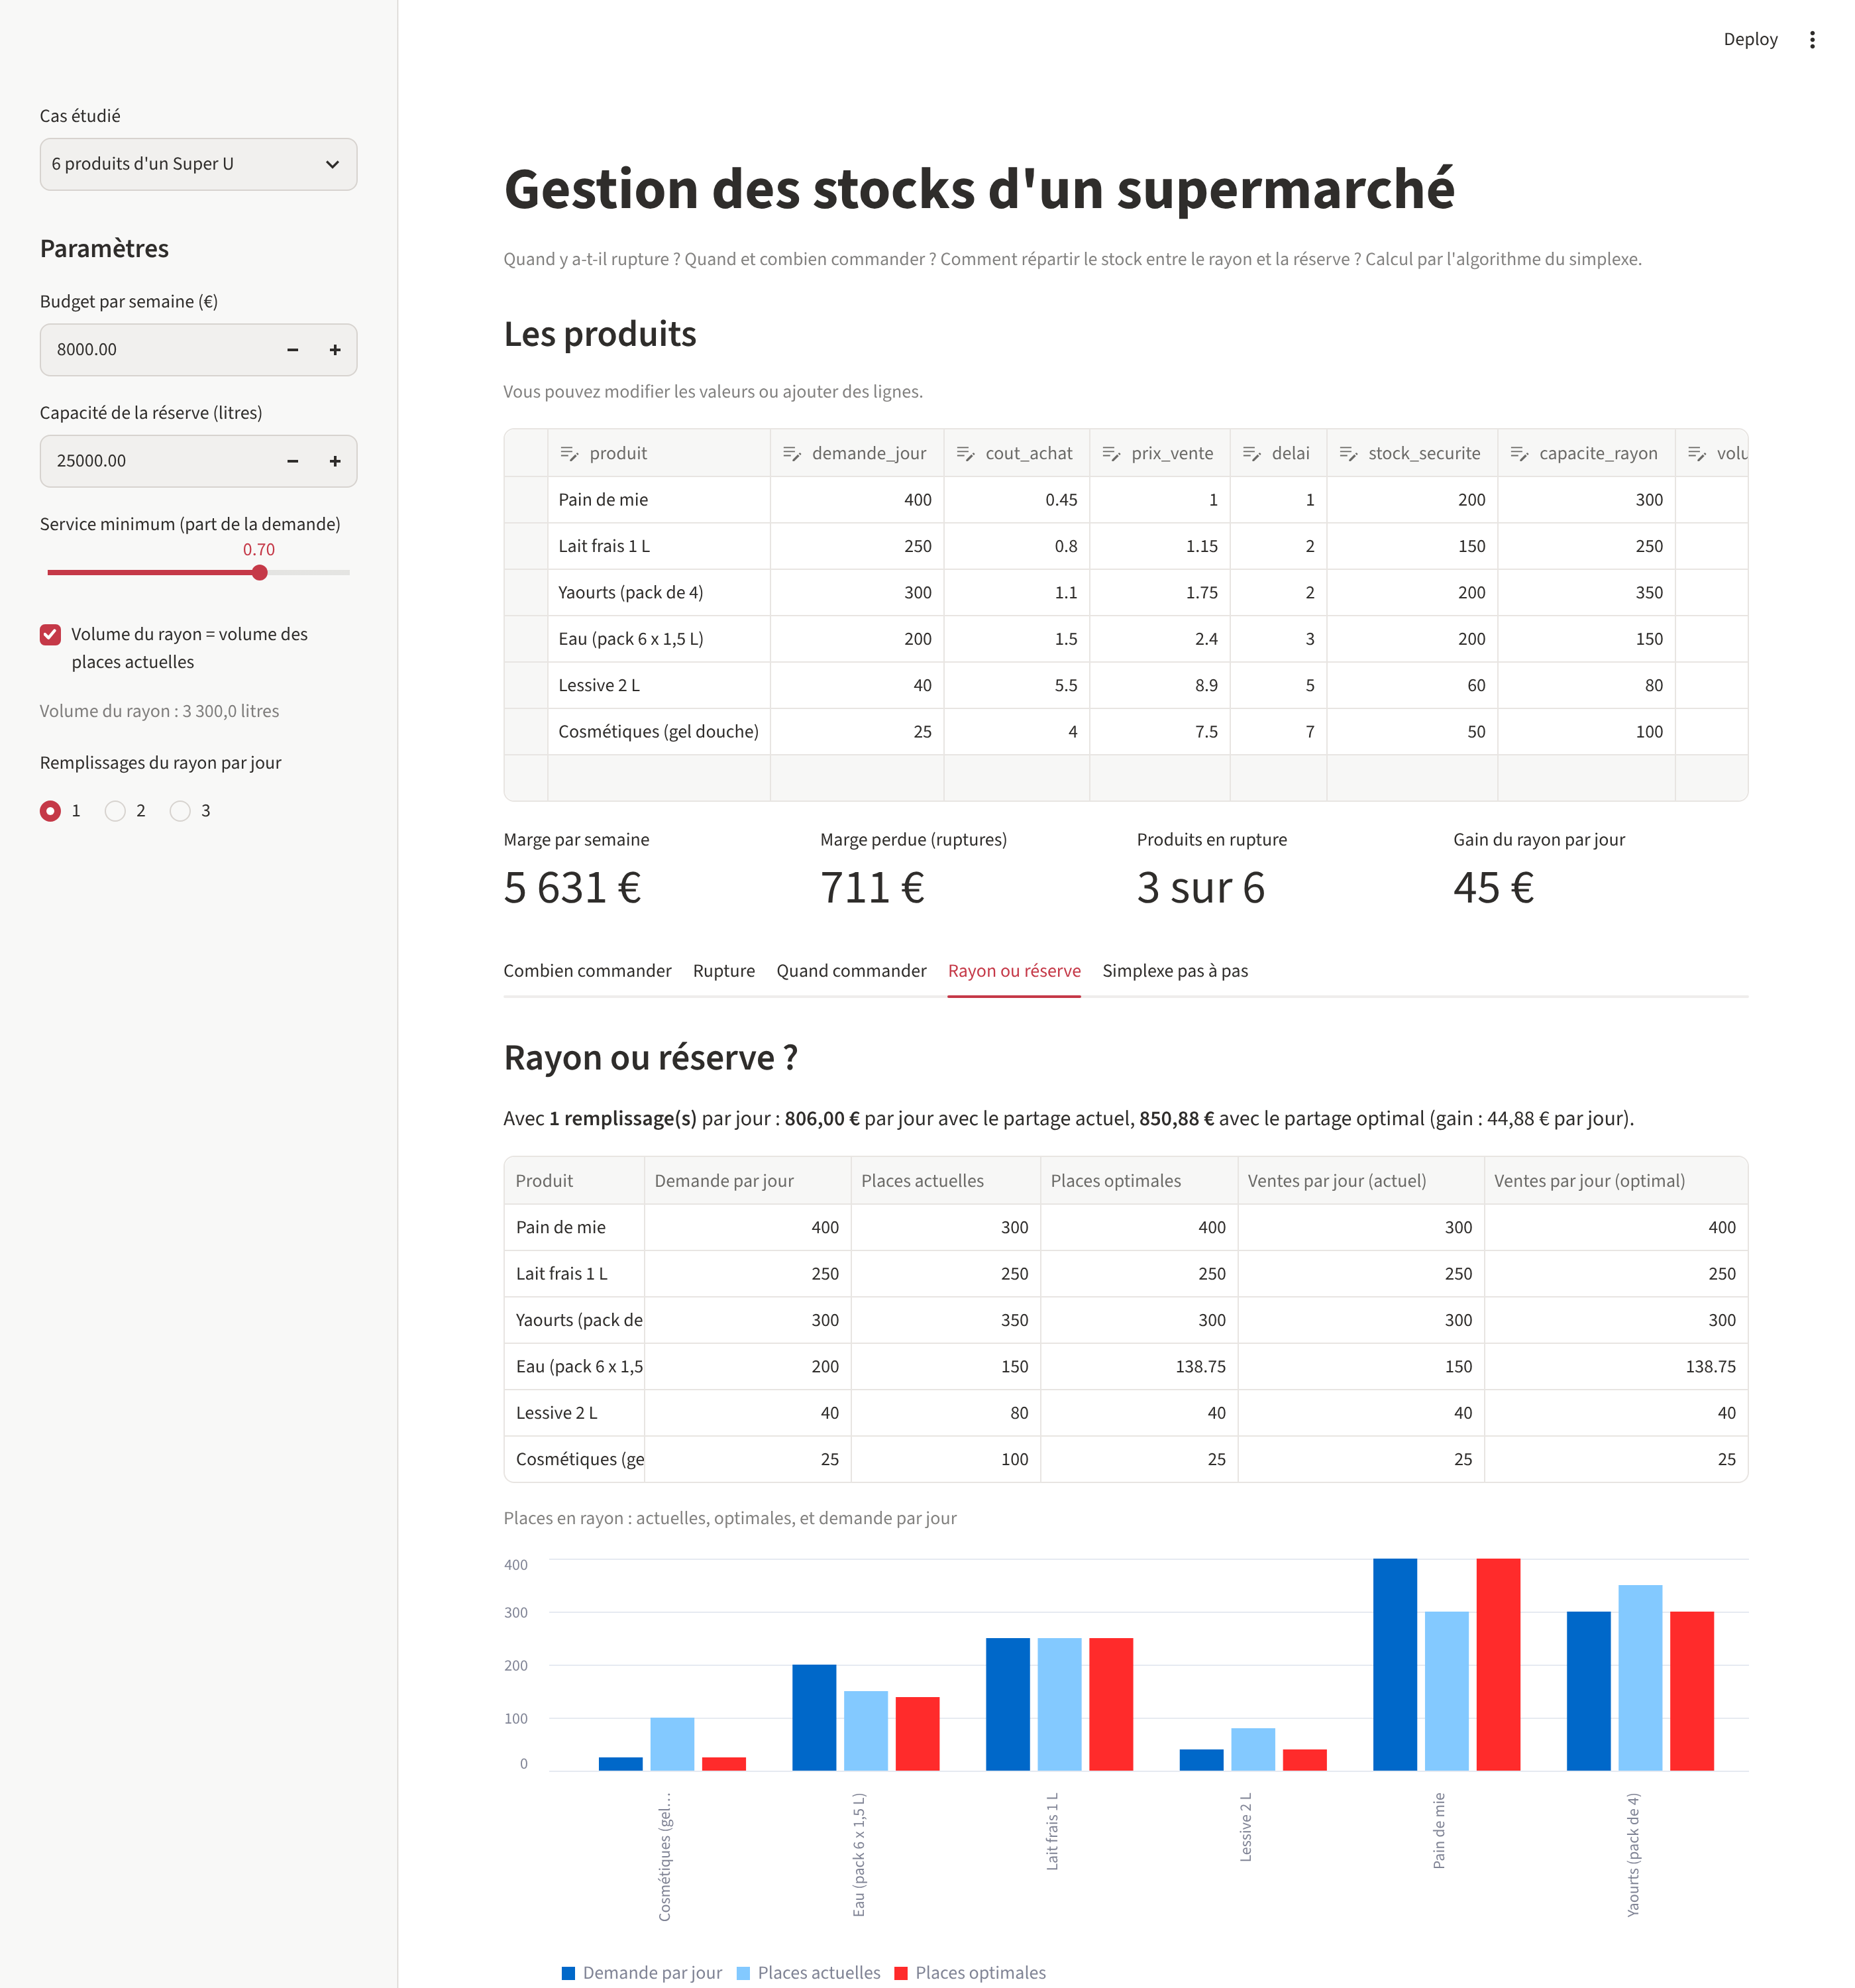
\includegraphics[width=0.74\linewidth]{app_streamlit.png}
\caption{L'application Streamlit sur les six produits, onglet « Rayon ou réserve »}
\label{fig:streamlit}
\end{figure}

\subsection{Vérification sur le cas à deux produits}
Avant de lui faire confiance, on vérifie que l'application retrouve les calculs de la
partie 2. La commande \texttt{python application.py --deux-produits} affiche exactement :
\begin{itemize}
\item les trois tableaux du simplexe « commandes », avec les mêmes pivots (4 puis 0,5) ;
\item la solution $a = 100$, $b = 50$, $Z = 550\eur$, et les écarts 40 et 90 ;
\item les jours couverts 5 et 2,5, donc les ruptures le samedi et le mercredi, et 570\eur{}
  de marge perdue ;
\item le calendrier : samedi pour A, vendredi pour B ;
\item le partage du rayon : 10 et 20 places, $Z = 130\eur$ (160\eur{} avec deux
  remplissages).
\end{itemize}
Ces contrôles sont automatisés dans \texttt{test\_modele.py} (huit tests, tous réussis). À
titre de contrôle supplémentaire, 30 magasins tirés au hasard (de 2 à 300 produits, soit
60 programmes linéaires) ont aussi été résolus avec le solveur SciPy (Virtanen et al.,
2020) : l'écart avec notre simplexe est de l'ordre de $10^{-9}$. Le solveur n'est utilisé
que pour ce contrôle, pas dans l'application.

\subsection{Application aux six produits d'un Super U}

\subsubsection*{Les données}
\begin{table}[H]
\centering\small
\caption{Données des six produits (hypothèses)}\label{tab:donnees6}
\begin{tabular}{@{}llrrrrrrr@{}}
\toprule
$i$ & Produit & $d_i$ & $c_i$ & $p_i$ & $m_i$ & $v_i$ & $R_i$ & $L_i$ \\
\midrule
1 & Pain de mie            & 400 & 0,45 & 1,00 & 0,55 & 3   & 300 & 1 \\
2 & Lait frais 1 L         & 250 & 0,80 & 1,15 & 0,35 & 1,2 & 250 & 2 \\
3 & Yaourts (pack de 4)    & 300 & 1,10 & 1,75 & 0,65 & 1   & 350 & 2 \\
4 & Eau (pack 6 x 1,5 L)   & 200 & 1,50 & 2,40 & 0,90 & 10  & 150 & 3 \\
5 & Lessive 2 L            & 40  & 5,50 & 8,90 & 3,40 & 2,5 & 80  & 5 \\
6 & Cosmétiques (gel douche) & 25 & 4,00 & 7,50 & 3,50 & 0,5 & 100 & 7 \\
\bottomrule
\end{tabular}

\vspace{3pt}
\footnotesize $d_i$ : demande par jour ; $c_i$ : coût d'achat (€) ; $p_i$ : prix de vente (€) ;
$m_i$ : marge unitaire (€) ; $v_i$ : volume (litres) ;\\ $R_i$ : places actuelles en rayon ;
$L_i$ : délai de livraison (jours).
\end{table}

Paramètres : budget de 8\,000\eur{} par semaine, réserve de 25\,000 litres (25 m\textsuperscript{3}),
service minimum de 70\,\%, rayon de 3\,300 litres (le volume des places actuelles), livraison
le lundi matin, un remplissage du rayon par jour. Servir toute la demande coûterait
9\,310\eur{} et occuperait 27\,388 litres : comme dans le cas à deux produits, le magasin ne
peut pas tout commander.

\subsubsection{Combien commander ?}
Le service minimum de 70\,\% fait partie du modèle : le minimum coûte 6\,517\eur, occupe
19\,171,25 litres et rapporte déjà 4\,439,40\eur{} de marge. Il reste 1\,483\eur{} de budget
et 5\,828,75 litres à répartir. On note $e_1$ le budget non dépensé, $e_2$ les litres libres
en réserve, et $e_3$ à $e_8$ la demande non servie des produits 1 à 6. Le simplexe
s'arrête après huit pivots :

\begin{table}[H]
\centering\small
\caption{Les huit pivots successifs}\label{tab:pivots}
\begin{tabular}{@{}clrlrrrl@{}}
\toprule
Étape & Entrante & $\Delta_j$ & Sortante & Rapport & Pivot & $Z'$ & Lecture \\
\midrule
1 & $z_6$ & 3,50 & $e_8$ & 52,5 & 1 & 183,75 & cosmétiques au plafond \\
2 & $z_5$ & 3,40 & $e_7$ & 84 & 1 & 469,35 & lessive au plafond \\
3 & $z_4$ & 0,90 & $e_6$ & 420 & 1 & 847,35 & eau au plafond \\
4 & $z_3$ & 0,65 & $e_1$ & 164,55 & 1,10 & 954,30 & yaourts : le budget est épuisé \\
5 & $z_1$ & 0,28 & $z_3$ & 402,22 & 0,41 & 1\,068,57 & le pain remplace les yaourts \\
6 & $e_7$ & 3,32 & $e_2$ & 5,44 & 34,17 & 1\,086,64 & moins de lessive, la réserve sature \\
7 & $e_6$ & 0,93 & $e_3$ & 111,39 & 3,33 & 1\,190,61 & moins d'eau, pain au plafond \\
8 & $e_2$ & 0,003 & $e_7$ & 185,83 & 0,03 & 1\,191,15 & lessive de nouveau au plafond \\
\bottomrule
\end{tabular}
\end{table}

Les quatre premiers pivots servent les produits dans l'ordre de leur marge unitaire, jusqu'à
épuiser le budget. L'étape 5 corrige ce choix : le pain rapporte moins par unité que les
yaourts (0,55 contre 0,65), mais il coûte beaucoup moins cher, donc il rapporte plus par
euro de budget. Les étapes 6 à 8 réduisent l'eau, qui consomme beaucoup de budget et de
réserve, au profit du pain. Comme dans la partie 2, la marge augmente à chaque pivot.

\begin{table}[H]
\centering\small
\caption{Solution optimale du programme « commandes »}\label{tab:solution}
\begin{tabular}{@{}lrrrrl@{}}
\toprule
Produit & Minimum & $z_i^{*}$ & $x_i^{*}$ & Plafond $H_i$ & Situation \\
\midrule
Pain de mie          & 1\,960 & 840    & 2\,800    & 2\,800 & plafond saturé \\
Lait frais 1 L       & 1\,225 & 0      & 1\,225    & 1\,750 & service minimum \\
Yaourts (pack de 4)  & 1\,470 & 0      & 1\,470    & 2\,100 & service minimum \\
Eau (pack 6 x 1,5 L) & 980    & 288,67 & 1\,268,67 & 1\,400 & entre les deux \\
Lessive 2 L          & 196    & 84     & 280       & 280    & plafond saturé \\
Cosmétiques          & 122,5  & 52,5   & 175       & 175    & plafond saturé \\
\bottomrule
\end{tabular}
\end{table}

\begin{figure}[H]
\centering
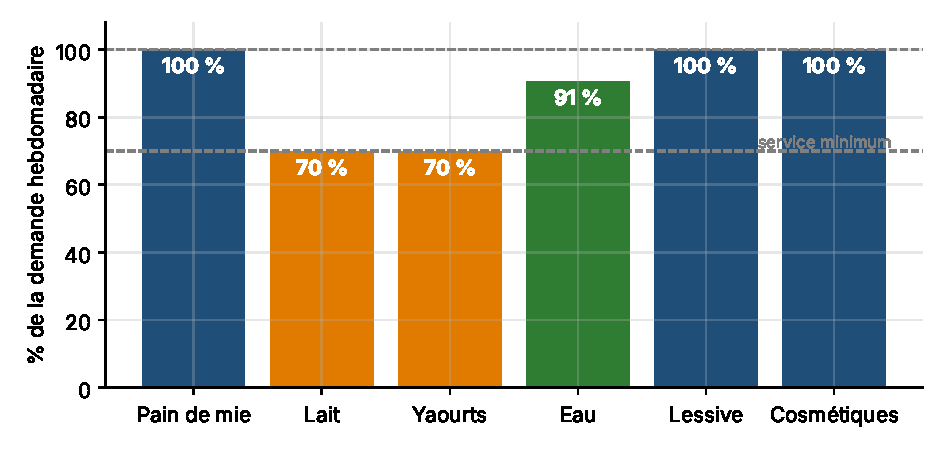
\includegraphics[width=0.74\linewidth]{solution_optimale.pdf}
\caption{Part de la demande hebdomadaire commandée à l'optimum
(bleu : plafond ; vert : entre les bornes ; orange : service minimum)}
\label{fig:solution}
\end{figure}

La marge optimale est $4\,439{,}40 + 1\,191{,}15 = \mathbf{5\,630{,}55}$\eur{} par semaine.
Le budget est saturé ($e_1 = 0$) ; la réserve ne l'est pas ($e_2 = 185{,}83$ litres libres).
Le simplexe a retrouvé de lui-même le bon critère : la marge par euro dépensé
$m_i / c_i$ (pain 1,22 ; cosmétiques 0,88 ; lessive 0,62 ; eau 0,60 ; yaourts 0,59 ; lait
0,44). Les trois premiers sont servis entièrement, l'eau reçoit le budget restant, les deux
derniers restent au minimum.

\subsubsection{Quand y a-t-il rupture ?}
\begin{table}[H]
\centering\small
\caption{Ruptures prévues par le programme (livraison le lundi matin)}\label{tab:ruptures}
\begin{tabular}{@{}lrrrlr@{}}
\toprule
Produit & $x_i^{*}$ & Écart (non servi) & Jours couverts & Rupture & Marge perdue \\
\midrule
Pain de mie          & 2\,800    & 0      & 7,0 & aucune            & 0 \\
Lait frais 1 L       & 1\,225    & 525    & 4,9 & vendredi soir & 183,75\eur \\
Yaourts (pack de 4)  & 1\,470    & 630    & 4,9 & vendredi soir & 409,50\eur \\
Eau (pack 6 x 1,5 L) & 1\,268,67 & 131,33 & 6,3 & dimanche          & 118,20\eur \\
Lessive 2 L          & 280       & 0      & 7,0 & aucune            & 0 \\
Cosmétiques          & 175       & 0      & 7,0 & aucune            & 0 \\
\midrule
Total                &           &        &     &                   & 711,45\eur \\
\bottomrule
\end{tabular}
\end{table}

\begin{figure}[H]
\centering
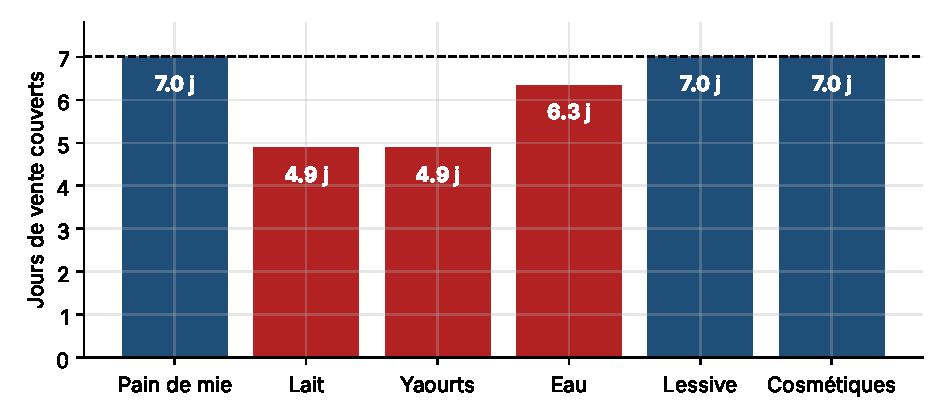
\includegraphics[width=0.72\linewidth]{ruptures.pdf}
\caption{Nombre de jours de vente couverts par la commande optimale (rouge : rupture avant
la fin de la semaine)}
\label{fig:ruptures}
\end{figure}

Comme dans le cas à deux produits, les ruptures se lisent dans les variables d'écart : le
lait et les yaourts manquent à partir du vendredi soir et tout le week-end, l'eau le
dimanche. Ce sont des ruptures que le magasin \textit{choisit}, parce que ce sont celles qui
coûtent le moins de marge par euro économisé. La marge perdue, 711,45\eur{} par semaine,
est l'écart entre la marge si tout était servi (6\,342\eur) et la marge optimale
(5\,630,55\eur).

\subsubsection{Quand commander ?}
\begin{table}[H]
\centering\small
\caption{Calendrier de commande pour une livraison le lundi matin}\label{tab:calendrier}
\begin{tabular}{@{}lrlrr@{}}
\toprule
Produit & Délai $L_i$ & Jour de commande & Stock de sécurité $SS_i$ & Point de commande $s_i$ \\
\midrule
Pain de mie          & 1 jour  & dimanche          & 200 & 600 \\
Lait frais 1 L       & 2 jours & samedi            & 150 & 650 \\
Yaourts (pack de 4)  & 2 jours & samedi            & 200 & 800 \\
Eau (pack 6 x 1,5 L) & 3 jours & vendredi          & 200 & 800 \\
Lessive 2 L          & 5 jours & mercredi          & 60  & 260 \\
Cosmétiques          & 7 jours & lundi précédent   & 50  & 225 \\
\bottomrule
\end{tabular}
\end{table}

\subsubsection{Rayon ou réserve ?}
Le rayon actuel est mal partagé : 100 places pour 25 ventes par jour de cosmétiques, mais
seulement 300 places pour 400 ventes de pain de mie et 150 pour 200 d'eau. Le programme
« rayon » partage les 3\,300 litres entre les six produits ; son simplexe s'arrête après
sept pivots.

\begin{table}[H]
\centering\small
\caption{Les sept pivots du programme « rayon » ($n = 1$)}\label{tab:pivotsrayon}
\begin{tabular}{@{}clrlrrrl@{}}
\toprule
Étape & Entrante & $\Delta_j$ & Sortante & Rapport & Pivot & $Z$ & Lecture \\
\midrule
1 & $r_6$ & 3,50 & $e_7$ & 25 & 1 & 87,50 & cosmétiques : toute la demande \\
2 & $r_5$ & 3,40 & $e_6$ & 40 & 1 & 223,50 & lessive : toute la demande \\
3 & $r_4$ & 0,90 & $e_5$ & 200 & 1 & 403,50 & eau : toute la demande \\
4 & $r_3$ & 0,65 & $e_4$ & 300 & 1 & 598,50 & yaourts : toute la demande \\
5 & $r_1$ & 0,55 & $e_1$ & 295,83 & 3 & 761,21 & pain : le rayon est plein \\
6 & $e_5$ & 0,93 & $e_2$ & 31,25 & 3,33 & 790,38 & moins d'eau, pain complet \\
7 & $r_2$ & 0,24 & $e_3$ & 250 & 1 & 850,88 & lait : toute la demande \\
\bottomrule
\end{tabular}
\end{table}

\begin{table}[H]
\centering\small
\caption{Partage actuel et partage optimal du rayon ($n = 1$)}\label{tab:rayon}
\begin{tabular}{@{}lrrrrr@{}}
\toprule
 & Demande & \multicolumn{2}{c}{Places en rayon} & \multicolumn{2}{c}{Marge par jour} \\
\cmidrule(lr){3-4}\cmidrule(lr){5-6}
Produit & par jour & actuelles & optimales & actuelle & optimale \\
\midrule
Pain de mie          & 400 & 300 & 400    & 165,00 & 220,00 \\
Lait frais 1 L       & 250 & 250 & 250    & 87,50  & 87,50 \\
Yaourts (pack de 4)  & 300 & 350 & 300    & 195,00 & 195,00 \\
Eau (pack 6 x 1,5 L) & 200 & 150 & 138,75 & 135,00 & 124,88 \\
Lessive 2 L          & 40  & 80  & 40     & 136,00 & 136,00 \\
Cosmétiques          & 25  & 100 & 25     & 87,50  & 87,50 \\
\midrule
Total                &     &     &        & 806,00\eur & 850,88\eur \\
\bottomrule
\end{tabular}
\end{table}

\begin{figure}[H]
\centering
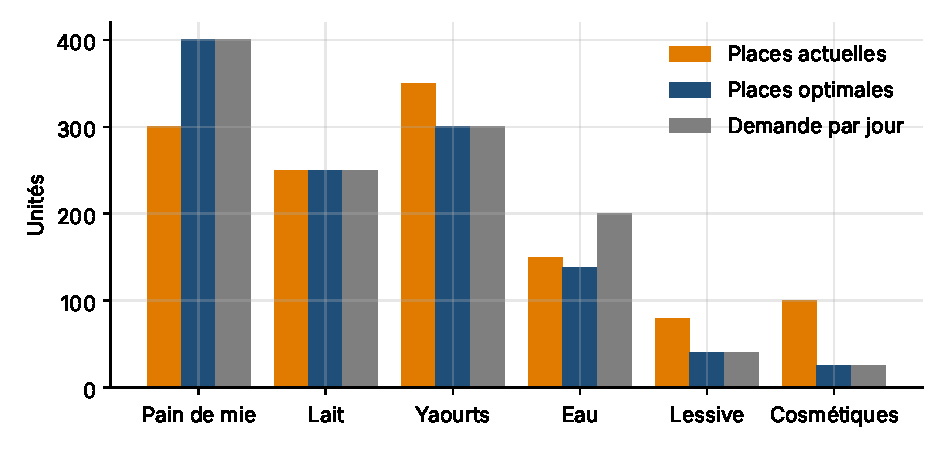
\includegraphics[width=0.74\linewidth]{rayon.pdf}
\caption{Places en rayon : partage actuel, partage optimal et demande d'une journée}
\label{fig:rayon}
\end{figure}

Le simplexe reprend la place gaspillée (cosmétiques, lessive, yaourts) et la donne au pain de
mie, qui passe de 300 à 400 places. Le gain est de $850{,}88 - 806{,}00 = 44{,}88\eur$ par
jour, soit environ 16\,400\eur{} par an, sans agrandir le rayon. Le seul produit encore en
rupture en rayon est l'eau (138,75 places pour 200 ventes), parce que c'est celui qui
rapporte le moins par litre de rayon ($0{,}90 / 10 = 0{,}09\eur$).

Avec deux remplissages par jour (\texttt{--remplissages 2}), il suffit de $d_i / 2$ places
par produit, soit 1\,956 litres. Le simplexe donne 906\eur{} par jour : toute la demande est
servie, le rayon n'est plus saturé, et l'agrandir serait inutile. Le gain est de
$906 - 806 = 100\eur$ par jour.

\subsection{Passage à l'échelle}
L'application est testée sur des magasins de 10 à 1\,000 produits, générés au hasard
(\texttt{--aleatoire}). Le budget y est fixé à 85\,\% du coût de la demande et la réserve à
90\,\% de son volume, comme dans le cas à six produits où le budget est inférieur à ce qu'il
faudrait pour tout servir.

\begin{table}[H]
\centering
\caption{L'application sur des magasins de plus en plus grands}\label{tab:echelle}
\small\setlength{\tabcolsep}{4pt}
\begin{tabular}{@{}rrrrrrr@{}}
\toprule
Produits & Tableau & Pivots & Temps & Marge par semaine & En rupture & Gain du rayon par jour \\
\midrule
6    & $8 \times 15$        & 15    & $< 0{,}1$ s & 5\,631\eur     & 3 sur 6        & 45\eur \\
10   & $12 \times 23$       & 17    & $< 0{,}1$ s & 25\,872\eur    & 7 sur 10       & 499\eur \\
100  & $102 \times 203$     & 164   & 0,05 s      & 162\,402\eur   & 47 sur 100     & 2\,889\eur \\
300  & $302 \times 603$     & 516   & 0,4 s       & 538\,942\eur   & 133 sur 300    & 9\,246\eur \\
1\,000 & $1\,002 \times 2\,003$ & 1\,648 & environ 8 s & 1\,920\,246\eur & 498 sur 1\,000 & 31\,340\eur \\
\bottomrule
\end{tabular}
\end{table}

« Tableau » est la taille du tableau du simplexe « commandes », et « Pivots » le nombre total
des deux programmes. Les temps sont ceux d'un ordinateur ordinaire. Le nombre de pivots reste de l'ordre de
1,5 à 2 fois le nombre de produits : l'algorithme ne parcourt qu'une toute petite partie
des sommets du programme admissible, ce qui le rend utilisable sur de grands magasins.
Les résultats se lisent comme dans le cas à deux produits ; seul le nombre de lignes change.
Comme les données sont tirées au hasard, ces chiffres montrent que l'application tient la
charge, pas ce qui se passerait dans un magasin réel.

% ------------------------------------------------------------------ 4
\section{Discussion : limites}

\textbf{Des données imaginaires.} Les conclusions chiffrées valent pour ces hypothèses. La
méthode, elle, s'applique à des données réelles : il suffit de remplacer le fichier des
produits.

\textbf{Une demande certaine.} La programmation linéaire suppose que la demande est connue.
En réalité elle varie d'un jour à l'autre, et les livraisons peuvent être en retard. Le
stock de sécurité sert à couvrir cet aléa, mais son niveau n'est pas optimisé par le modèle.

\textbf{Des quantités non entières.} Le simplexe donne 1\,268,67 packs d'eau et 138,75
places en rayon. À cette échelle, l'arrondi ne change presque rien : à 1\,268 packs, le
budget et la réserve restent respectés et la marge baisse de moins d'un euro.

\textbf{Deux programmes séparés.} Le programme « commandes » et le programme « rayon » sont
résolus l'un après l'autre. Le second suppose que la marchandise est disponible en réserve,
ce qui n'est pas vrai le week-end pour le lait et les yaourts. Un programme unique serait
plus juste, mais ses tableaux seraient plus grands.

\textbf{Un simplexe maison.} L'algorithme programmé est celui du cours : il est lisible et
suffit jusqu'à quelques milliers de produits. Au-delà, un solveur professionnel serait plus
rapide, mais on perdrait la possibilité d'afficher et d'expliquer chaque tableau.

\textbf{Un seul critère.} Le modèle maximise la marge. Un client qui ne trouve pas de lait
le samedi peut aller faire toutes ses courses ailleurs : ce coût d'image n'est pas compté.
Le service minimum de 70\,\% en tient compte de façon approximative.

% ------------------------------------------------------------------ 5
\section{Conclusion}
Ce dossier répond aux trois questions en deux temps : à la main sur un magasin de deux
produits, puis avec une application sur un nombre quelconque de produits.

\textbf{Quand y a-t-il rupture ?} Quand la quantité commandée est épuisée : elle couvre
$x_i^{*} / d_i$ jours, et la demande non servie se lit dans les variables d'écart du tableau
final. Avec deux produits, A manque à partir du samedi et B à partir du mercredi. Avec six
produits, le lait et les yaourts manquent à partir du vendredi soir et l'eau le dimanche.

\textbf{Quand et combien commander ?} Les quantités viennent du simplexe : 100 unités de A
et 50 de B (550\eur{} par semaine) pour deux produits, et 5\,630,55\eur{} par semaine pour
six produits, avec un budget entièrement dépensé. Les dates viennent des délais : on
commande de un à sept jours avant la livraison du lundi.

\textbf{Comment répartir le stock entre le rayon et la réserve ?} Un second programme
linéaire partage la place du rayon : 10 places pour A et 20 pour B (130\eur{} par jour au
lieu de 120), et 44,88\eur{} par jour de plus pour les six produits. Avec deux
remplissages par jour, toutes les ventes perdues en rayon disparaissent.

L'intérêt de la démarche est qu'elle se comprend en entier sur le cas à deux produits, et
que l'application ne fait ensuite rien d'autre que répéter les mêmes étapes à grande échelle.
Deux recommandations en découlent pour le magasin : remplir le rayon deux fois par jour, et
redistribuer les places du rayon en faveur des produits qui se vendent le plus.

% ------------------------------------------------------------------ biblio
\section*{Bibliographie}
\addcontentsline{toc}{section}{Bibliographie}
\begin{description}\setlength{\itemsep}{1pt}\small
\item \textit{Recherche opérationnelle et optimisation}, support de cours et travaux
  dirigés, Master 2, Université d'Angers.
\item Faure, R., Lemaire, B., et Picouleau, C. \textit{Précis de recherche opérationnelle}.
  Dunod.
\item Teghem, J. \textit{Recherche opérationnelle}. Ellipses.
\item Virtanen, P., et al. (2020). SciPy 1.0: fundamental algorithms for scientific
  computing in Python. \textit{Nature Methods}, 17, 261-272.
\end{description}

\section*{Annexe : le cœur de l'algorithme}
\addcontentsline{toc}{section}{Annexe : le cœur de l'algorithme}
Le simplexe de \texttt{simplexe.py} tient en quelques lignes. Il suit exactement les étapes
de la partie 2 : profits marginaux, variable entrante, rapports, variable sortante, pivot.

\begin{lstlisting}
while True:
    delta = profits_marginaux(tableau, couts, base)   # ligne Delta_j
    colonne = choisir_entrante(delta)                 # variable entrante
    if colonne is None:                               # optimum atteint
        break
    rapports = calculer_rapports(tableau, colonne)    # b_i / a_ij
    ligne = int(np.argmin(rapports))                  # variable sortante
    pivoter(tableau, ligne, colonne)                  # mise a jour
    base[ligne] = colonne
\end{lstlisting}

\end{document}
